%%%%%%%%%%%%%%%%%%%%%%%%%%%%%%%%%%%%
\section{Tool Support}
\label{sect:tool} %
%%%%%%%%%%%%%%%%%%%%%%%%%%%%%%%%%%%%

We realized our method as a tool in a Java software framework that we reported in previous works~\cite{le_domain_2018, le_jdomainapp_2017}. The tool is available at the git repository\footnote{\url{https://github.com/jdomainapp/jda-mbsl}}. It takes as input a configured unified model and semi-automatically generates as the output an interactive software prototype. This prototype is used by the development team to develop the domain model and, once this is completed, may also be reused to develop the production software.

\begin{figure*}[ht]
	\centering
	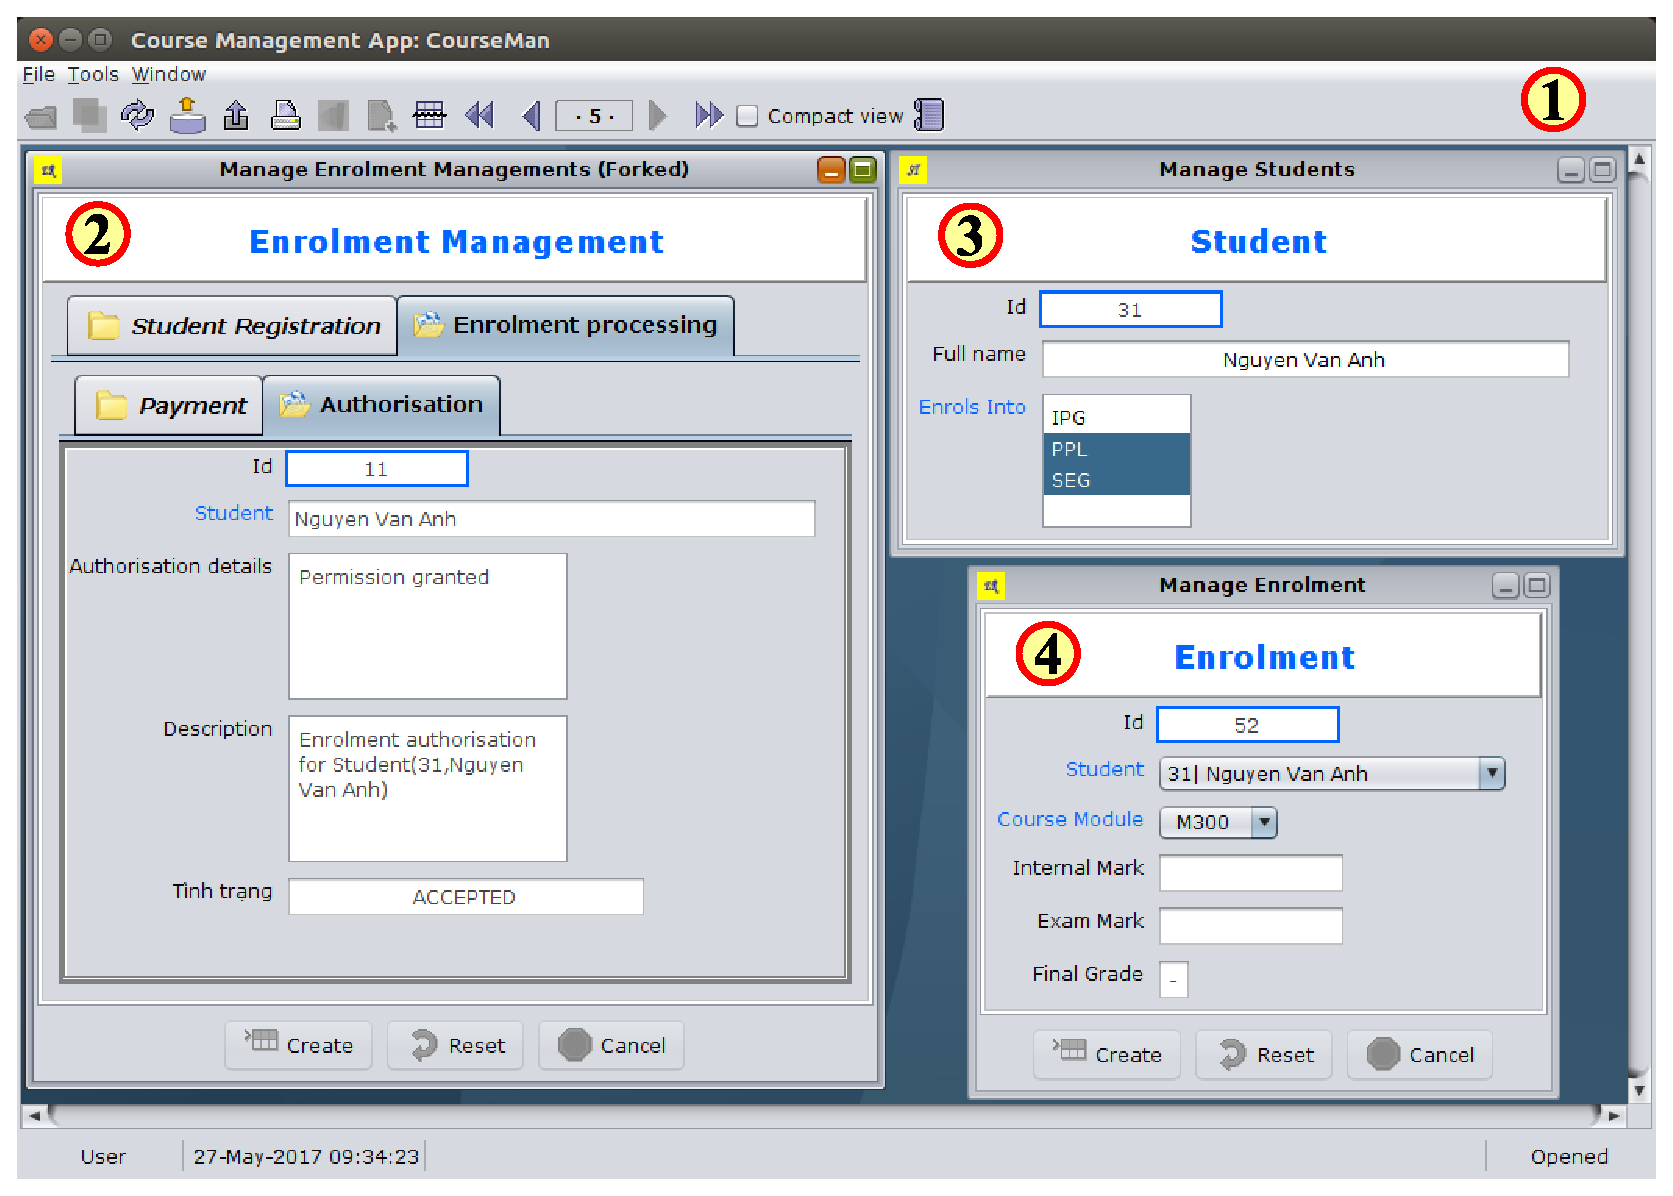
\includegraphics[scale=0.4]{software-tool}
	\caption{The GUI of \courseman~software generated by the tool: (1) desktop, 
		(2-4) the object UIs of \clazz{EnrolmentMgmt}, \clazz{Student}, and \clazz{Enrolment}.} %
	\label{fig:software-tool}
\end{figure*}

Conceptually, the tool consists of three key components: model manager, view manager, and object manager. First, \textbf{model manager} is responsible for registering the configured unified model and making it accessible to other components. 
Second, \textbf{view manager} is responsible for (1) automatically generating the entire GUI of the software from the unified model and (2) for handling the user interaction performed on this GUI. The GUI consists of a set of object UIs (one for each module's view), and a desktop for organising these UIs. For example, Figure~\ref{fig:software-tool} shows the generated GUI for one variant of the \courseman~unified model. The GUI contains three object UIs for \clazz{ModuleEnrolmentMgmt}, \clazz{ModuleStudent}, and \clazz{ModuleEnrolment}.
%Later in the Section~\ref{sect:eval-expressiveness}, we will demonstrate how the tool is used to generate 
Several other variants of the \courseman~unified model, as mentioned in Section~\ref{sect:behaviorPatterns}, could also be generated. 

Third, \textbf{object manager} is responsible for managing the run-time object pool of each domain class and for providing a generic object storage component for storing/retrieving the objects to/from an external storage. As of this writing, the tool supports both file-based and relational database storage. The relational data model is automatically generated from the unified model the first time the software is run.
